%% =====================================================================
%% SAGE-MM --- Graphical Abstract (Elsevier), landscape ~2.5:1.
%% Build:  pdflatex graphical_abstract.tex   -> graphical_abstract.pdf
%% (scripts/build.sh also builds it and exports a PNG.)
%% =====================================================================
\documentclass[border=4pt]{standalone}
\usepackage{tikz}
\usepackage{helvet}
\renewcommand{\familydefault}{\sfdefault}
\usetikzlibrary{arrows.meta,positioning,backgrounds,fit}

\definecolor{hdr}{RGB}{31,78,121}      % deep blue
\definecolor{boxb}{RGB}{225,236,246}   % light blue fill
\definecolor{statb}{RGB}{232,232,232}  % grey fill (static, non-adaptive)
\definecolor{ctrlb}{RGB}{252,232,205}  % amber fill (the adaptive part)
\definecolor{good}{RGB}{34,120,60}
\definecolor{warn}{RGB}{193,110,20}
\definecolor{ink}{RGB}{40,40,40}

\begin{document}
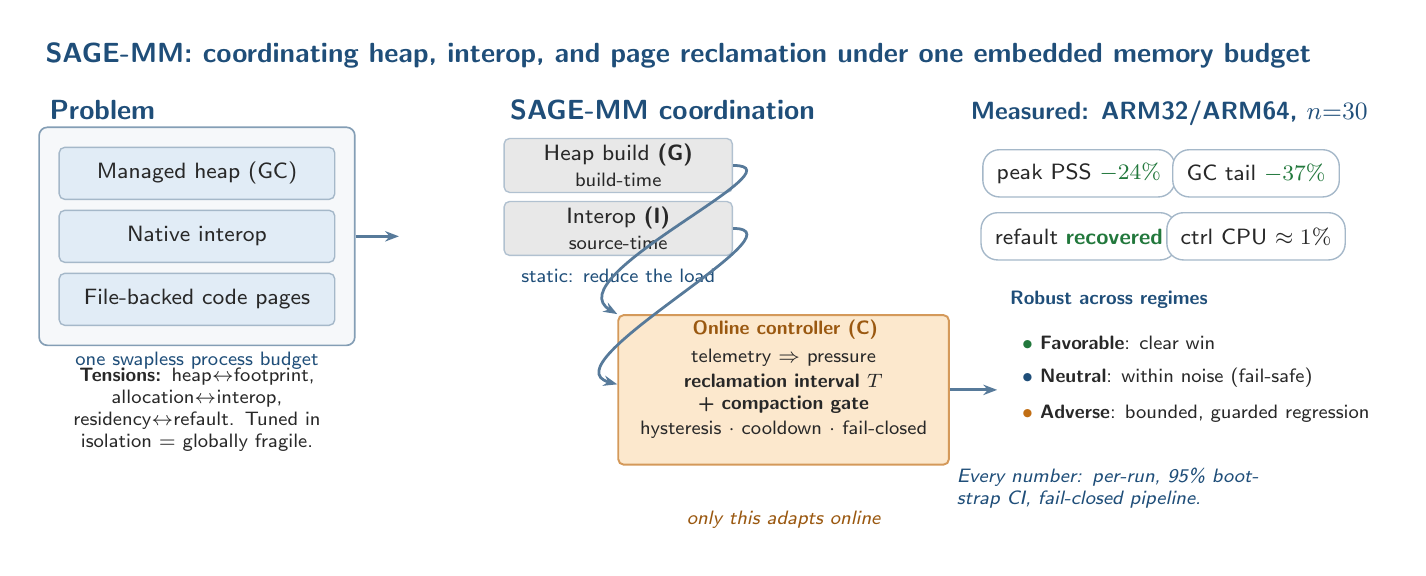
\begin{tikzpicture}[
  font=\footnotesize, ink,
  every node/.style={inner sep=2pt},
  panel/.style={rounded corners=3pt, draw=hdr!55, line width=0.6pt},
  layer/.style={rounded corners=2pt, draw=hdr!40, fill=boxb, line width=0.5pt,
                minimum width=3.5cm, minimum height=0.66cm, align=center},
  stat/.style={rounded corners=2pt, draw=hdr!35, fill=statb, line width=0.5pt,
               minimum width=2.9cm, minimum height=0.62cm, align=center},
  ctrl/.style={rounded corners=2pt, draw=warn!70, fill=ctrlb, line width=0.7pt,
               align=center},
  chip/.style={rounded corners=6pt, draw=hdr!40, fill=white, line width=0.5pt,
               minimum height=0.6cm, align=center, inner xsep=5pt},
  flow/.style={-{Stealth[length=5pt]}, line width=1pt, hdr!75},
]
\useasboundingbox (0,0) rectangle (17.4,6.6);

%% ---- Title strip ----
\node[anchor=west, hdr, font=\bfseries\normalsize] at (0.15,6.25)
  {SAGE-MM: coordinating heap, interop, and page reclamation under one embedded memory budget};

%% =========================================================
%% Panel A --- the problem: one process budget, three layers
%% =========================================================
\node[anchor=north west, hdr, font=\bfseries] at (0.2,5.75) {Problem};
\node[layer] (heap) at (2.15,4.75) {Managed heap (GC)};
\node[layer] (interop) at (2.15,3.95) {Native interop};
\node[layer] (pages) at (2.15,3.15) {File-backed code pages};
\begin{scope}[on background layer]
  \node[panel, fill=hdr!4, fit=(heap)(interop)(pages),
        inner sep=7pt, label={[hdr,font=\scriptsize]below:one swapless process budget}] (procbox) {};
\end{scope}
\node[align=center, font=\scriptsize, text width=3.9cm] at (2.15,1.75)
  {\textbf{Tensions:} heap$\leftrightarrow$footprint,
   allocation$\leftrightarrow$interop, residency$\leftrightarrow$refault.
   Tuned in isolation $=$ globally fragile.};

%% =========================================================
%% Panel B --- SAGE-MM coordination
%% =========================================================
\node[anchor=north west, hdr, font=\bfseries] at (6.05,5.75) {SAGE-MM coordination};

\node[stat] (G) at (7.5,4.85) {Heap build \textbf{(G)}\\\scriptsize build-time};
\node[stat] (I) at (7.5,4.05) {Interop \textbf{(I)}\\\scriptsize source-time};
\node[align=center, font=\scriptsize, hdr] at (7.5,3.45) {static: reduce the load};

\node[ctrl, minimum width=4.2cm, minimum height=1.9cm] (C) at (9.6,2.0) {};
\node[anchor=north, font=\bfseries\scriptsize, warn!80!black] at (C.north) {\,Online controller \textbf{(C)}};
\node[align=center, font=\scriptsize] at (9.6,1.95)
  {telemetry $\Rightarrow$ pressure\\[1pt]
   \textbf{reclamation interval $T$}\\
   \textbf{+ compaction gate}\\[1pt]
   \scriptsize hysteresis $\cdot$ cooldown $\cdot$ fail-closed};
\node[font=\scriptsize\itshape, warn!80!black, align=center] at (9.6,0.35)
  {only this adapts online};

\draw[flow] (G.east) to[out=0,in=150] (C.north west);
\draw[flow] (I.east) to[out=0,in=165] ([yshift=2pt]C.west);

%% panel-to-panel arrows
\draw[flow] (procbox.east) -- ++(0.55,0) node[midway,above,font=\scriptsize]{};
\draw[flow] (C.east) -- ++(0.6,0);

%% =========================================================
%% Panel C --- measured outcome
%% =========================================================
\node[anchor=north west, hdr, font=\small\bfseries] at (11.9,5.75)
  {Measured: ARM32/ARM64, $n{=}30$};

\node[chip, minimum width=2.05cm] (s1) at (13.35,4.75) {peak PSS \textbf{\textcolor{good}{$-24\%$}}};
\node[chip, minimum width=2.05cm] (s2) at (15.6,4.75) {GC tail \textbf{\textcolor{good}{$-37\%$}}};
\node[chip, minimum width=2.05cm] (s3) at (13.35,3.95) {refault \textbf{\textcolor{good}{recovered}}};
\node[chip, minimum width=2.05cm] (s4) at (15.6,3.95) {ctrl CPU \textbf{$\approx1\%$}};

\node[anchor=west, font=\scriptsize\bfseries, hdr] at (12.4,3.15) {Robust across regimes};
\node[anchor=west, font=\scriptsize] at (12.55,2.6)
  {\textcolor{good}{$\bullet$} \textbf{Favorable}: clear win};
\node[anchor=west, font=\scriptsize] at (12.55,2.15)
  {\textcolor{hdr}{$\bullet$} \textbf{Neutral}: within noise (fail-safe)};
\node[anchor=west, font=\scriptsize] at (12.55,1.7)
  {\textcolor{warn}{$\bullet$} \textbf{Adverse}: bounded, guarded regression};

\node[align=left, font=\scriptsize\itshape, text width=3.9cm, hdr] at (13.75,0.75)
  {Every number: per-run, 95\% bootstrap CI, fail-closed pipeline.};

\end{tikzpicture}
\end{document}
